\documentclass{beamer}

%%%%%%%%%%%%%Solarized Theme%%%%%%%%%%%%%%%
\usecolortheme[light,accent=cyan]{solarized}
\beamertemplatenavigationsymbolsempty

%%%%%Packages%%%%%
\usepackage{graphicx}
\usepackage{hyperref}
\usepackage{colortbl, xcolor}
\usepackage{booktabs}
\usepackage{standalone}
\usepackage{color}
\usepackage{pgfplots}

\usepackage{tikz}
\usetikzlibrary{positioning, decorations.markings}
\usetikzlibrary{calc}

\begin{document}
 
\begin{frame}
    \centering
    \LARGE \textbf{Nikoleta E. Glynatsi} \\
    \vfill
    \includegraphics[width=.4\textwidth]{static/me.jpg}
    % \vfill
    % \Large Vincent Knight \& Jonathan Gillard
\end{frame}

\begin{frame}
    % \begin{columns}
    %     \begin{column}{.5\textwidth}
            \centering
            \Large \textbf{Vincent Knight \&} \textbf{Jonathan Gillard} \\
            \vspace{3mm}
            \includegraphics[width=.7\textwidth]{static/supervisors.jpg}
        % \end{column}
        % \begin{column}{.5\textwidth}
        %     \centering
        %     \Large \textbf{Jonathan Gillard} \\
        %     \vspace{3mm}
        %     \includegraphics[width=.7\textwidth]{static/Jonathan-Gillard.jpg}
        % \end{column}
    % \end{columns}
\end{frame}

\begin{frame}
    \centering
    \Large \textbf{GAME THEORY}
\end{frame}

\begin{frame}
    \centering
    \includegraphics[width=.2\textwidth]{static/players} \hspace{.6cm}
    \includegraphics[width=.2\textwidth]{static/actions} \hspace{.6cm}
    \includegraphics[width=.2\textwidth]{static/objective}
\end{frame}

\begin{frame}
    \centering
    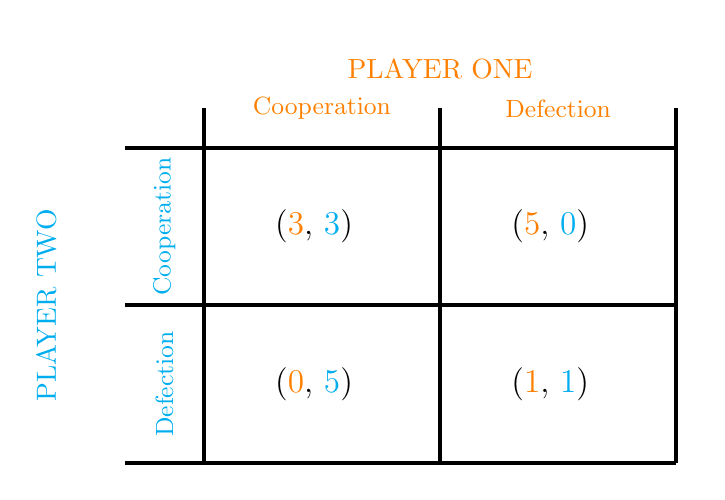
\begin{tikzpicture}
        \tikzstyle{state}=[minimum width=1cm, font=\boldmath];
        
        \node at (3, 3) {\textcolor{orange}{PLAYER ONE}};
        \node[rotate=90] at (-2, 0) {\textcolor{cyan}{PLAYER TWO}};
        %horizontal lines
        \pause

        \draw[-, line width=2pt, ultra thick] (-1, -2) -- (6, -2) node[right] {};
        \draw[-, line width=2pt, ultra thick] (-1, 0) -- (6, 0) node[right] {};
        \draw[-, line width=2pt, ultra thick] (-1, 2) -- (6, 2) node[right] {};
    
        % vertical lines
        \draw[-, line width=2pt, ultra thick] (0,-2) -- (0, 2.5) node[above] {};
        \draw[-, line width=2pt, ultra thick] (3,-2) -- (3, 2.5) node[above] {};
        \draw[-, line width=2pt, ultra thick] (6,-2) -- (6, 2.5) node[above] {};
    
        % % dashed lines
        % \draw[dashed, line width=1pt, ultra thick] (0, 2) -- (4, 0) node[right] {};
        % \draw[dashed, line width=1pt, ultra thick] (4, 2) -- (8, 0) node[right] {};
        % \draw[dashed, line width=1pt, ultra thick] (0, 0) -- (4, -2) node[right] {};
        % \draw[dashed, line width=1pt, ultra thick] (4, 0) -- (8, -2) node[right] {};
    
        % player's actions
        \node[circle, ultra thick] (0) at (1.5, 2.5) [state] {\small \textcolor{orange}{Cooperation}};
        \node[circle, ultra thick] (0) at (4.5, 2.5) [state] {\small \textcolor{orange}{Defection}};
        \node[circle, ultra thick, rotate=90] (0) at (-0.5, 1) [state] {\small \textcolor{cyan}{Cooperation}};
        \node[circle, ultra thick, rotate=90] (0) at (-0.5, -1) [state] {\small \textcolor{cyan}{Defection}};

        \pause
    
        % payoffs
        \node[circle, ultra thick] (0) at (1.4, 1) [state] {\large {(\textcolor{orange}3, \textcolor{cyan}3)}};
        \node[circle, ultra thick] (0) at (4.4, 1) [state] {\large {(\textcolor{orange}5, \textcolor{cyan}0)}};
        \node[circle, ultra thick] (0) at (4.4, -1) [state] {\large {(\textcolor{orange}1, \textcolor{cyan}1)}};
        \node[circle, ultra thick] (0) at (1.4, -1) [state] {\large {(\textcolor{orange}0, \textcolor{cyan}5)}};
        \end{tikzpicture}
\end{frame}

\begin{frame}
    \centering
    \includegraphics[width=.19\textwidth]{static/examine} \hspace{.6cm}
    \includegraphics[width=.19\textwidth]{static/computer} \hspace{.6cm}
    \includegraphics[width=.19\textwidth]{static/train}
\end{frame}

\begin{frame}
    \centering
    \includegraphics[width=.6\textwidth]{static/hands}
\end{frame}

\end{document}

